\section{LIDA Framework}
\label{sec:lida}
LIDA is both the name of a cognitive model and a software framework implementing
most parts of the LIDA model.
Explain the important parts of the framework and how they are used and implemented

\subsection{The LIDA model}
\begin{figure}[h!tb]
\centering
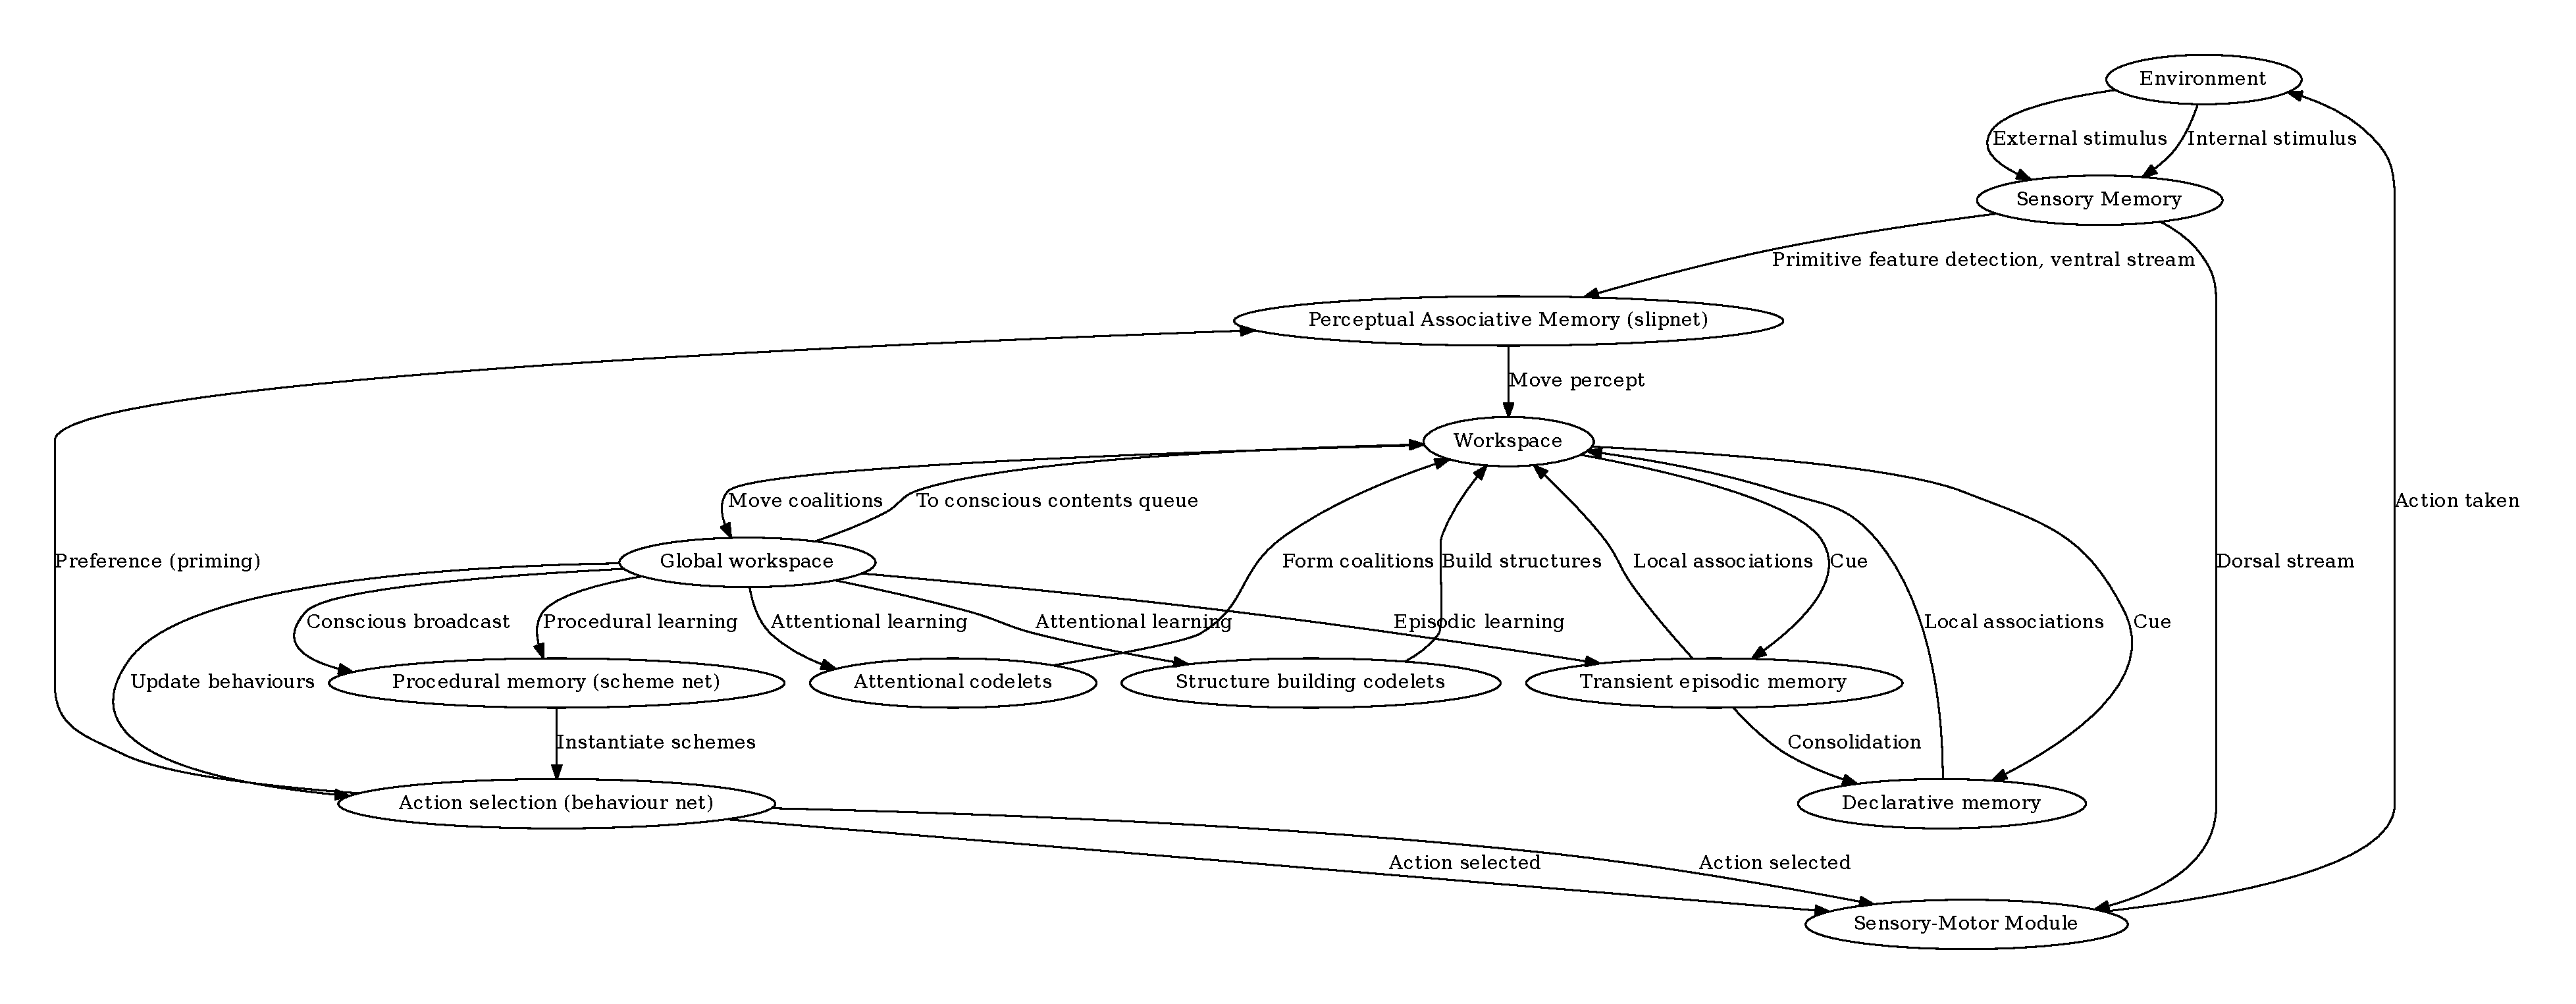
\includegraphics[angle=90, height=0.85\textheight]{graphics/lida-cycle.pdf}
\caption{The LIDA cycle}
\label{fig:lida-cycle}
\end{figure}

The LIDA model is a conceptual and computational model that describes cognition.
It is based on the General Workspace Theory, which is a theory to describe
functional consciousness. It incorporates and accounts for a large number of
psychological and neuropsychological theories.

\subsubsection{The LIDA cognitive cycle}
The computational model of LIDA views the artificial agent's ``life'' as a
series of cognitive cycles. A high-level, simplified view of how this cognitive
cycle is modeled in LIDA can be seen in figure \ref{fig:lida-cycle}.

The cognitive cycle itself is subdivided into three separate phases; the
understanding phase, the consciousness phase and the action selection phase.

\paragraph{Understanding phase}
In the understanding phase sensory input is tagged with semantic meaning. First
low-level feature detectors in the Sensory Memory are run, running on the
incoming stimuli. The output from these is passed onto the Perceptual
Associative Memory. There higher-level feature detectors are run, which
recognise abstracted entities like objects, events, actions, etc. The output of
these is sent to the Workspace, from where it is pushed to both the Transient
Episodic Memory and the Declarative Memory. Local associations generated from
these memory modules are combined with the percept to generate a Current
Situational Model, which is the agent's ``inner map'' of how the world looks.

\paragraph{Attention phase}
Parts of the Current Situational Model is composited together to coalitions by
Attention Codelets. These coalitions are put into the Global Workspace.
From the Global Workspace a codelet selects the coalition in most need of
conscious attention and broadcasts this.

\paragraph{Action selection phase}
The Action Selection module takes in possible action schemes from the
Procedural Memory, and selects one of these according to a competetive process.
The selected action scheme is sent to the Sensory-Motor Memory, where it is
executed.

Learning is also done in the action selection phase. In the Perceptual
Associative Memory new entities and associations are created and old ones are
reinforced during this phase. In the Transient Episodic Memory events from the
broadcast from the Global Workspace are stored. The Procedural Memory stores
new possible action schemes from the broadcast, and reinforces old ones.

\subsubsection{The workspace}
The workspace is composed of three main modules; the Current Situational Model,
Scratchpad and the Conscious Contents Queue.

\paragraph{Current Situational Model} This is where the internal ``map'' of the
agent is represented. This contains current events that are linked to
associations. Various structure-building codelets running in the Workspace are
responsible for building these.

\paragraph{Scratchpad} The Scratchpad is used for temporary storage for the
codelets while they build up structures before moving into Current Situational
Model.

\paragraph{Conscious Contents Queue}
This contains a list of previous broadcasts, which allows LIDA to take time
into account, and work on things that happen in the time domain.

